\documentclass[11pt, fleqn]{article}

\usepackage{amsmath}
\usepackage{amssymb}
\usepackage{amsthm}
\usepackage{mathtools}
\usepackage{hyperref}
\usepackage{ulem}
\usepackage{enumitem}
\usepackage[left=0.75in, right=0.75in, bottom=0.75in]{geometry}
\usepackage{graphicx}
% \usepackage{float}
\usepackage{floatrow}

\usepackage{sectsty}
\sectionfont{\centering}

\usepackage[perpage]{footmisc}

\usepackage{fancyhdr}
\pagestyle{fancy}
\fancyhf{}
\lhead{190100044 \& 190100055}
\rhead{CS 215: Assignment 2}
\renewcommand{\footrulewidth}{1.0pt}
\cfoot{Page \thepage}

\setlength{\parindent}{0em}
\renewcommand{\arraystretch}{2}%

\title{Assignment 2: CS 215}
\author{
\begin{tabular}{|c|c|}
     \hline
     Devansh Jain & Harshit Varma \\
     \hline
     190100044 & 190100055 \\
     \hline
\end{tabular}
}
\date{September 6, 2020}

\begin{document}

\maketitle
\tableofcontents
\thispagestyle{empty}
\setcounter{page}{0}


\newpage
\section*{Question 1}
\addcontentsline{toc}{section}{Question 1}
\setcounter{equation}{0}

Given that $X_1, \dots, X_n$ are $n$ Independent Identically distributed random variables with cdf $F_X(x)$ and pdf $f_X(x) = F_X'(x)$.\\

To determine cdf and pdf for $Y_1 = \text{max}(X_1, \dots, X_n)$
\begin{equation*}
\begin{split}
    F_{Y_1}(x) &= P(Y_1 \le x) \\
        &= \prod_{i=1}^{n} P(X_i \le x) \hspace{3em} (\text{As $Y_1$ = max($X_i$s), $Y_1 \ge X_i \  \forall i$}) \\
        &= P(X \le x)^n \hspace{3em} (\text{$X_i$s are identically distributed}) \\
    \Aboxed{F_{Y_1}(x) &= F_X(x)^n} \\
    \Aboxed{f_{Y_1}(x) &= n \cdot F_X(x)^{n-1} \cdot f_X(x)} \hspace{3em} (\text{Differentiation w.r.t $x$}) \\
\end{split}
\end{equation*}

To determine cdf and pdf for $Y_2 = \text{min}(X_1, \dots, X_n)$
\begin{equation*}
\begin{split}
    F_{Y_2}(x) &= P(Y_2 \le x) = 1 - P(Y_2 \ge x) \\
        &= 1 - \prod_{i=1}^{n} P(X_i \ge x) \hspace{3em} (\text{As $Y_2$ = min($X_i$s), $Y_2 \le X_i \ \forall i$}) \\
        &= 1 - (P(X \ge x))^n \hspace{3em} (\text{$X_i$s are identically distributed}) \\
        &= 1 - (1 - P(X \le x))^n \\
    \Aboxed{F_{Y_2}(x) &= 1 - (1 - F_X(x))^n} \\
    \Aboxed{f_{Y_2}(x) &= n \cdot (1 - F_X(x))^{n-1} \cdot f_X(x)} \hspace{3em} (\text{Differentiation w.r.t $x$}) \\
\end{split}
\end{equation*}

The cdf and pdf of $Y_1 = \text{max}(X_1, \dots, X_n)$ are $F_X(x)^n$ and $n \cdot F_X(x)^{n-1} \cdot f_X(x)$ respectively. \\
The cdf and pdf of $Y_2 = \text{min}(X_1, \dots, X_n)$ are $1 - (1 - F_X(x))^n$ and $n \cdot (1 - F_X(x))^{n-1} \cdot f_X(x)$ respectively.







\newpage
\section*{Question 2}
\addcontentsline{toc}{section}{Question 2}
\setcounter{equation}{0}

\subsection*{Part 1}
It's given that $X$ belongs to a Gaussian Mixture Model.\\
$$ f_X(x) = \sum_{i=1}^{k}p_i \mathcal{N}(\mu_i, \sigma_i^2) $$
Throughout the rest of this question, we shall use $G_i$ for denoting $\mathcal{N}(\mu_i, \sigma_i^2) $.
\subsubsection*{Calculating E($X$):}
We know that $E(X) = \int_{-\infty}^{\infty} x G_i dx = \mu_i$ (Expection of a Gaussian)\\
Thus,
$$
\begin{aligned}
    E(X) &= \int_{-\infty}^{\infty}x f_X(x) dx\\
    &= \int_{-\infty}^{\infty} x \sum_{i=1}^{k}p_i G_i dx\\
    &= \sum_{i=1}^{k}p_i \int_{-\infty}^{\infty} x G_i dx\\
    &= \boxed{ \sum_{i=1}^{k}p_i \mu_i }
\end{aligned}
$$
\subsubsection*{Caluclating Var($X$):}
We know that:
$$ 
Var(X) = E((X-\mu)^2) = E(X^2) - E(X)^2 = E(X^2) - \mu^2 $$
and,
$$
\begin{aligned}
Var(X) &= \sigma_i^2 = E(X^2)-\mu_i^2 \text{ for a Gaussian } G_i \\
\text{Thus, } E(X^2) &= \int_{-\infty}^{\infty} x^2 G_i dx = \sigma_i^2+\mu_i^2
\end{aligned}
$$
We shall now calculate $E(X^2)$
$$
\begin{aligned}
    E(X^2) &= \int_{-\infty}^{\infty} x^2 \sum_{i=1}^{k}p_i G_i dx\\
    &= \sum_{i=1}^{k}p_i \int_{-\infty}^{\infty} x^2 G_i dx\\
    &= \sum_{i=1}^{k}p_i (\sigma_i^2 + \mu_i^2)
\end{aligned}
$$
Thus, now we have:
$$
Var(X) = E(X^2)-\mu^2 = \boxed{ \sum_{i=1}^{k}p_i (\sigma_i^2 + \mu_i^2) - (\sum_{i=1}^{k}p_i \mu_i)^2 }
$$
\\
\subsubsection*{Caluclating the MGF:}
By the definition of the MGF, $\phi_X (t) = E(e^{tX})$\\
We also know that for a gaussian $G_i$, we have $\phi_X (t) = \int_{-\infty}^{\infty}e^{tx} G_i dx = \exp(\mu_i t + \frac{(\sigma_i t)^2}{2})$\\
Thus for the given $X$,
$$
\begin{aligned}
    \phi_X (t) &= E(e^{tX}) \\
    &= \int_{-\infty}^{\infty}e^{tX} \sum_{i=1}^{k}p_i G_i dx\\
    &= \sum_{i=1}^{k}p_i \int_{-\infty}^{\infty}e^{tX} G_i dx\\
    &= \boxed{\sum_{i=1}^{k}p_i\exp(\mu_i t + \frac{(\sigma_i t)^2}{2})}
\end{aligned}
$$
\subsection*{Part II}
It is given that $Z = \sum_{i=1}^{k}p_iX_i $ where $X_i \thicksim G_i$ are independent random variables.\\
By the properties of Gaussian distribution $G_i$ we know that:\\
$$
\begin{aligned}
E(X_i) &= \mu_i\\
Var(X_i) &= \sigma_i^2\\
\end{aligned}
$$
\subsubsection*{Calculating E($Z$):}
$$
\begin{aligned}
    E(Z) &= E( \sum_{i=1}^{k}p_iX_i)\\
    &= \sum_{i=1}^{k}p_i E(X_i) \hspace{3em} (\text{Linearity of Expectation})\\
    &= \boxed{ \sum_{i=1}^{k}p_i\mu_i }
\end{aligned}
$$
\subsection*{Calculating Var($Z$)}
$$
\begin{aligned}
    Var(Z) &= Var( \sum_{i=1}^{k}p_iX_i)\\
    &= \sum_{i=1}^{k}p_i^2 Var(X_i) \hspace{3em} (\text{as $\{ X_i\}_{i=1}^k$ are independent and $Var(aX) = a^2Var(X)$})\\
    &= \boxed{ \sum_{i=1}^{k}p_i^2\sigma_i^2 }
\end{aligned}
$$

\subsection*{Calculating the MGF}
We know that for a Gaussian $X_i \thicksim G_i$, we have:
$$ \phi_{X_{i}} (t) = \int_{-\infty}^{\infty}e^{tx} G_i dx = \exp(\mu_i t + \frac{(\sigma_i t)^2}{2}) $$
We also know the following properties of $\phi_{X}(t)$:
$$ \phi_{(aX)}(t) = \phi_{X}(at) $$
$$ \phi_{X+Y}(t) =  \phi_{X}(t) \phi_{Y}(t) \text{ for independent X, Y }$$
Thus, using the above 2 properties, and the fact that $\{ X_i\}_{i=1}^k$ are independent,
$$
\begin{aligned}
    \phi_{Z}(t) &= \prod_{i=1}^{k}\phi_{(p_iX_i)}(t)\\
    &= \prod_{i=1}^{k}\phi_{X_i}(p_it)\\
    &= \prod_{i=1}^{k}\exp(\mu_i p_i t + \frac{(\sigma_i p_i t)^2}{2}) \hspace{1em} (\text{as } X_i \thicksim G_i ) \\
    &= \boxed{\exp(t\sum_{i=1}^k\mu_i p_i + \frac{t^2}{2}\sum_{i=1}^{k}p_i^2\sigma_i^2} \hspace{1em} (\text{as } \exp(a)\exp(b) = \exp(a+b)) 
\end{aligned}
$$
\subsection*{Calculating the PDF}
The obtained MGF of $Z$ is same as that of a gaussian of mean $\mu = \sum_{i=1}^k(\mu_i p_i)$ and variance $\sigma^2 = \sum_{i=1}^{k}p_i^2\sigma_i^2$\\
Thus, $Z \thicksim \mathcal{N}(\mu, \sigma^2)$. (Using the Moment Generating Function (MGF) Uniqueness Theorem\footnote{For a given random variable, the MGF and PMF \textbf{uniquely} determine each other.})\\
Therefore, the PDF of Z will be:
$$ \boxed{f_Z(z) = \frac{1}{\sigma \sqrt{2\pi}} \exp\bigg(-\frac{(z-\mu)^2}{2\sigma^2}\bigg)} $$


\newpage
\section*{Question 3}
\addcontentsline{toc}{section}{Question 3}
\setcounter{equation}{0}
\textbf{To prove:}
$$ 
P(X-\mu \ge \tau) \le \frac{\sigma^2}{\sigma^2+\tau^2} \hspace{2em} \text{for } \tau > 0
$$
$$ 
P(X-\mu \ge \tau) \ge 1 - \frac{\sigma^2}{\sigma^2+\tau^2} \hspace{2em} \text{for } \tau < 0
$$
We shall prove some lemmas before coming to the actual proof:\\
(Consider $X$ to be a random variable and $a \ge 0$.)
\begin{enumerate}
    \item $P(X \ge a) = P(X+b \ge a+b)$\\
    \label{lemma1}
    Note that $ (X \ge a) \iff (X+b \ge a+b) $,
    thus this directly leads to the above statement.
    \item $ P(X^2 \ge a^2) \ge P(X \ge a) $\\
    \label{lemma2}
    This is because of the fact that:
    $$ X^2 \ge a^2 \Rightarrow |X| \ge a \Rightarrow (X > a) \lor (X < -a) $$
    Thus, $ P(X^2 \ge a^2) = P(X > a) + P(X < -a)$. \\
    As probabilities are always  $\ge 0$, $ P(X^2 \ge a^2) \ge P(X > a) $
\end{enumerate}
Markov's Inequality states that, for $a > 0$ and a random variable $X$ which always takes positive values, we have:
$$ P(X \ge a) \le \frac{E(X)}{a} $$
Consider a random variable $Y := X - \mu$ and $Z := Y + b$ and consider the case where $\tau > 0$. \\
Also consider $b \ge 0$, thus we have $(\tau + b) \ge 0$\\
Thus, as $Z^2 \ge 0$ and $ (\tau + b)^2 > 0 $, we can apply the Markov's inequality these:
$$ P((Y+b)^2 \ge (\tau + b)^2) \le \frac{E((Y+b)^2)}{(\tau + b)^2} $$
Also, by Lemma \ref{lemma2}, we have $ P((Y+b)^2 \ge (\tau + b)^2) \ge P(Y+b \ge \tau + b) $.\\
By Lemma \ref{lemma1}, $ P((Y+b) \ge (\tau + b)) = P(Y \ge \tau) $\\
Now, using the linearity of the expectation operator,
$$
\begin{aligned}
    E((Y+b)^2) &= E(Y^2) + E(2Yb) + E(b^2)\\
    &= E(Y^2) + 2bE(Y) + b^2 \hspace{2em} \text{(expectation of a constant is the constant itself)}\\
    &= \sigma^2 + 0 + b^2 = \sigma^2 + b^2 \hspace{2em} (E((X-\mu)^2) = \sigma^2 \text{ and $ E(X-\mu) = 0 $)}
\end{aligned}
$$
Thus we have,
$$
    P(Y \ge \tau) \le \frac{\sigma^2 + b^2}{(\tau + b)^2}
$$
To further tighten the inequality, we need to minimize the function $ g(b) =  \frac{\sigma^2 + b^2}{(\tau + b)^2} $, solving $ g'(b) = 0 $ will yield us an extrema $b_0$:
$$ g'(b) = \frac{2b}{(\tau + b)^2} - \frac{2(\sigma^2 + b^2)}{(\tau + b)^3} $$
Equating it to zero, we get $ b_0 = \frac{\sigma^2}{\tau} $, furthermore as $g''(b) > 0$, this indeed is the minima.\\
Thus, after putting $Y = X - \mu$ and $b = b_0$, we get:
$$
    \boxed{P((X-\mu) \ge \tau) \le \frac{\sigma^2}{\sigma^2+\tau^2}} \hspace{2em} (\text{for } \tau > 0)
$$
Now, as $(X-\mu)^2 = (\mu - X)^2$, the inequality $ P((Y) \ge \tau) \le \frac{\sigma^2}{\sigma^2+\tau^2} $ is valid even for $Y = \mu -X$.\\
Thus for $ \tau < 0 $ we can still use the above result for $ -\tau $.\\
$$
\begin{aligned}
P((\mu - X) \ge (-\tau)) &\le \frac{\sigma^2}{\sigma^2+\tau^2}\\
P((X-\mu) < \tau) &\le \frac{\sigma^2}{\sigma^2+\tau^2}\\
1-P((X-\mu) \ge \tau) &\le \frac{\sigma^2}{\sigma^2+\tau^2} \hspace{1em} (P(X < a) = 1 - P(X \ge a))\\
\end{aligned}
$$
$$
\boxed{P((X-\mu) \ge \tau) \ge 1 - \frac{\sigma^2}{\sigma^2+\tau^2}} \hspace{1em} (\text{for } \tau < 0)
$$









\newpage
\section*{Question 4}
\addcontentsline{toc}{section}{Question 4}
\setcounter{equation}{0}

By definition, MGF of a random variable X for parameter t is $\phi_X(t) = \int_{-\infty}^{\infty} e^{tu} f_X(u) du$.\\

\begin{equation}
    \label{1}
    \begin{split}
        e^{-tx} \phi_X(t) &= \int_{-\infty}^{\infty} e^{t(u-x)} f_X(u) du \\
            &\ge \int_{-\infty}^{\infty} (1 + t(u-x)) f_X(u) du \hspace{3em} (e^x \ge (1 + x)) \\
    \end{split}
\end{equation}
\\
For $t \ge 0$,
\begin{equation}
    \begin{split}
        e^{-tx} \phi_X(t) &\ge \int_{x}^{\infty} (1 + t(u-x)) f_X(u) du \hspace{3em} (\text{From \ref{1}}) \\
            &\ge [\int_{x}^{\infty} f_X(u) du] + [t \cdot \int_{x}^{\infty} (u-x) f_X(u) du] \\
            &\ge P(X \ge x) + [t \cdot \int_{x}^{\infty} (u-x) f_X(u) du]
    \end{split}
\end{equation}
As $\quad t \ge 0;\quad u \ge x; \quad f_X(u) \ge 0 \  \forall u\in(-\infty, \infty), \quad$ we get
\begin{equation}
    \label{3}
    P(X \ge x) \le e^{-tx} \phi_X(t) \quad \forall t \ge 0
\end{equation}
\\
For $t \le 0$,
\begin{equation}
    \begin{split}
        e^{-tx} \phi_X(t) &\ge \int_{-\infty}^{x} (1 + t(u-x)) f_X(u) du \hspace{3em} (\text{From \ref{1}}) \\
            &\ge [\int_{-\infty}^{x} f_X(u) du] + [t \cdot \int_{-\infty}^{x} (u-x) f_X(u) du] \\
            &\ge P(X \le x) + [t \cdot \int_{-\infty}^{x} (u-x) f_X(u) du]
    \end{split}
\end{equation}
As $\quad t \le 0;\quad u \le x; \quad f_X(u) \ge 0 \  \forall u\in(-\infty, \infty), \quad$ we get
\begin{equation}
    P(X \le x) \le e^{-tx} \phi_X(t) \quad \forall t \ge 0
\end{equation}

\newpage
Now, $X = \sum_{i=1}^{n} X_i$, where $X_i$ are independent Bernoulli random variables with mean $p_i$.\\
$E(X) = \mu = \sum_{i=1}^{n} p_i$.\\
\begin{equation}
    \label{6}
    \begin{split}
        \phi_X(t) &= \prod_{i=1}^{n} \phi_{X_i}(t) \hspace{3em} (X_i \text{s are independent random variables}) \\
            &= \prod_{i=1}^{n} (1 - p_i + p_i e^{t}) \hspace{3em} (X_i \text{s are Bernoulli random variables}) \\
            &\le \prod_{i=1}^{n} (e^{p_i(e^t - 1)}) \hspace{3em} (e^x \ge (1 + x)) \\
            &\le exp(\sum_{i=1}^{n} p_i(e^t - 1)) \\
            &\le exp(\mu (e^t - 1)) \\
    \end{split}
\end{equation}
\begin{equation}
    \begin{split}
        P(X > (1 + \delta) \mu) &\le e^{-t \cdot ((1 + \delta) \mu)} \phi_X(t) \quad \forall t \ge 0 \hspace{3em} (\text{From \ref{3}}) \\
            &\le exp((-(1 + \delta) t \mu)) + \mu (e^t - 1)) \hspace{3em} (\text{From \ref{6}})
    \end{split}
\end{equation}
Therefore,
\begin{equation}
    \label{8}
    P(X > (1 + \delta) \mu) \le \frac{e^{\mu(e^t-1)}}{e^{(1+\delta)t\mu}} \quad \forall t \ge 0, \ \delta \ge 0
\end{equation}
To get a tighter bound, we need the minimum attainable value of the RHS of Eqn \ref{8}. \\
As $e^x$ is a monotonically increasing function, we need to minimize $(-(1 + \delta) t \mu)) + \mu (e^t - 1)$.\\
$\frac{d}{dt} ((-(1 + \delta) t \mu)) + \mu (e^t - 1)) = (\mu e^t - (1 + \delta) \mu) = 0 \quad \implies \quad t = ln(1 + \delta)$ \\
\begin{equation}
    P(X > (1 + \delta) \mu) \le \frac{e^{\mu\delta}}{e^{\mu(1+\delta)(ln(1 + \delta))}} \quad \forall \delta \ge 0 \\
\end{equation}










\newpage
\section*{Question 5}
\addcontentsline{toc}{section}{Question 5}
\setcounter{equation}{0}
\subsection*{Instructions for running the code:}
\begin{itemize}
    \item After extracting submitted file, look for a directory named \texttt{code}. 
    \item Within this, the code for this question is contained in a directory named \texttt{q5}.
    \item Run the file \texttt{q5a.m}, \texttt{q5b.m} and \texttt{q5c.m} for part (a), (b) and (c) respectively.
    \item The plots can be found in \texttt{./plots/}
    \item a\_*.png, b\_*.png and c.png are plots corresponding part (a), (b) and (c) respectively.
\end{itemize}

\subsection*{(a)}
\begin{figure}[H]
    \centering
    \begin{floatrow}
        \ffigbox[0.4\textwidth]{}
        {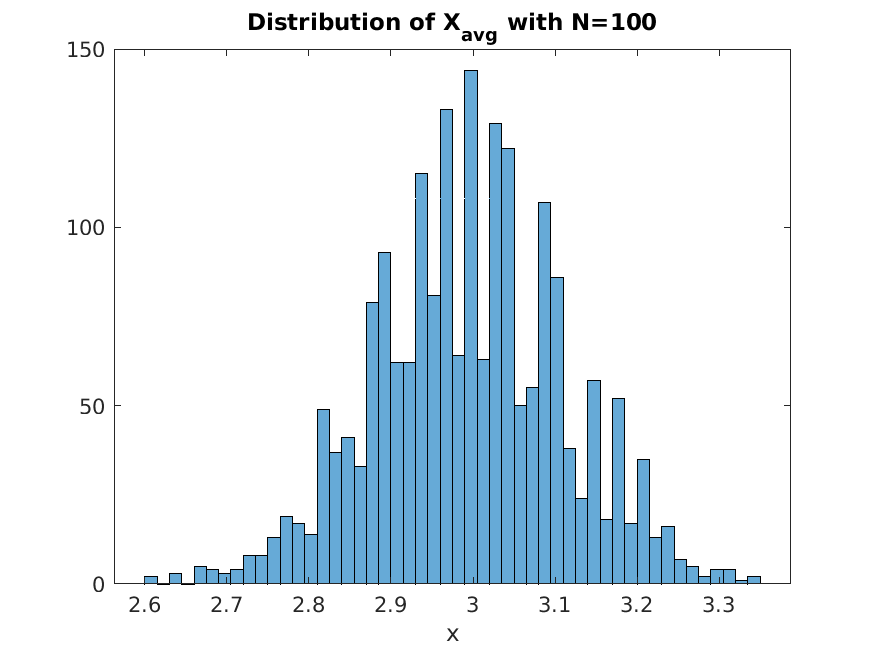
\includegraphics[height=0.4\textwidth]{a_100.png}}
        \ffigbox[0.4\textwidth]{}
        {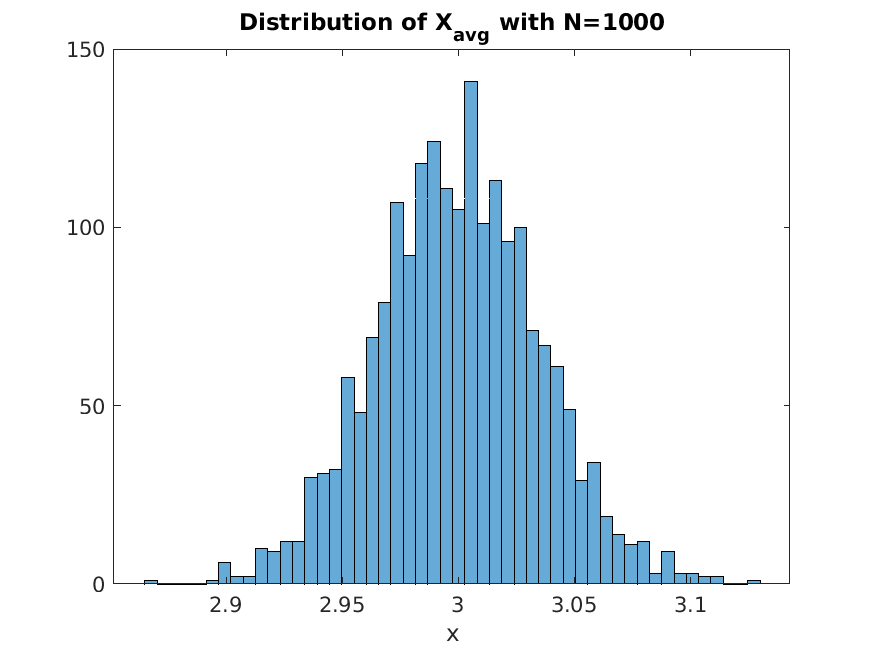
\includegraphics[height=0.4\textwidth]{a_1000.png}}
    \end{floatrow}
    \vspace{1em}
    \begin{floatrow}
        \ffigbox[0.4\textwidth]{}
        {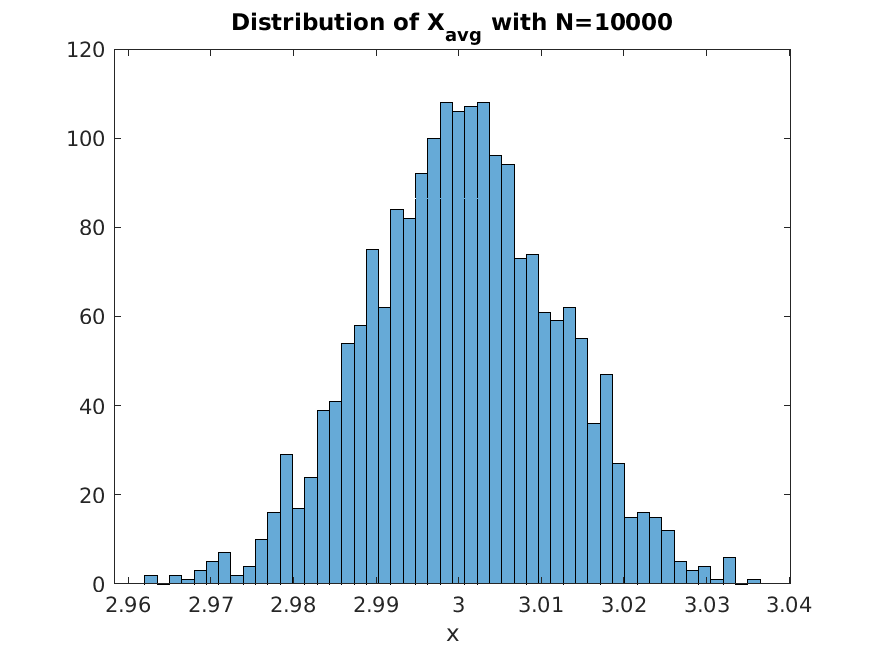
\includegraphics[height=0.4\textwidth]{a_10000.png}}
    \end{floatrow}
\end{figure}

\subsection*{(b)}
We also had to calculate the true mean $\mu$ and std. dev. $\sigma$ for getting the Gaussian curve.
\begin{equation*}
    \begin{split}
        \mu = E(X) &= \sum_{i=1}^{5} i \cdot f_{X_{avg}}(X_{avg} = i) = 1*0.05 + 2*0.4 + 3*0.15 + 4*0.3 + 5*0.1 = 3 \\
        \sigma^2 = Var(X) &= E((X-\mu)^2) = E((X-3)^2)= \sum_{i=1}^{5} (i - 3)^2 \cdot f_{X_{avg}}(X_{avg} = i) \\
            &= 4*0.05 + 1*0.4 + 0*0.15 + 1*0.3 + 4*0.1 = 1.3 \\
        \sigma &= \sqrt{1.3}
    \end{split}
\end{equation*}

\begin{figure}[H]
    \centering
    \begin{floatrow}
        \ffigbox[0.4\textwidth]{}
        {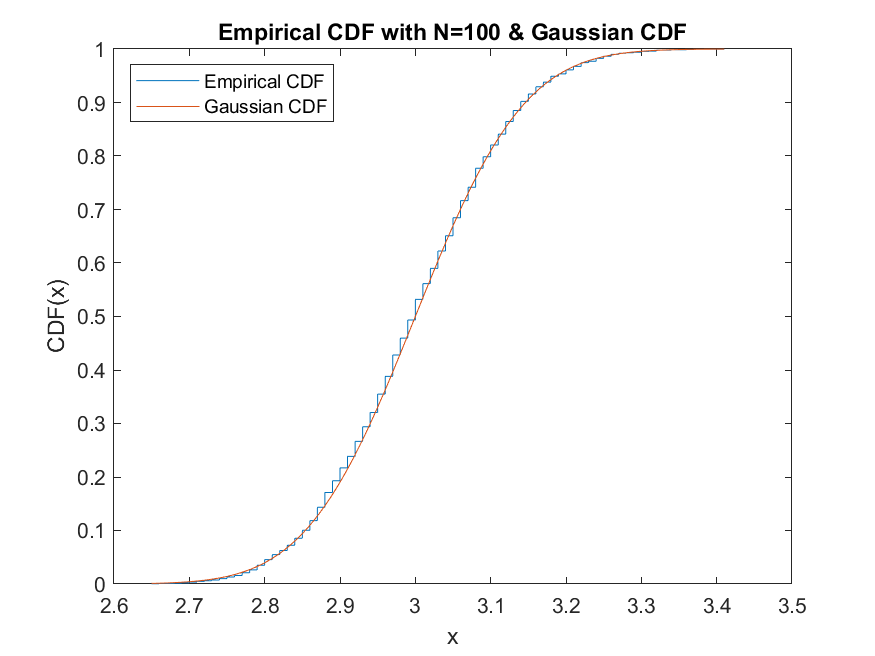
\includegraphics[height=0.4\textwidth]{b_100.png}}
        \ffigbox[0.4\textwidth]{}
        {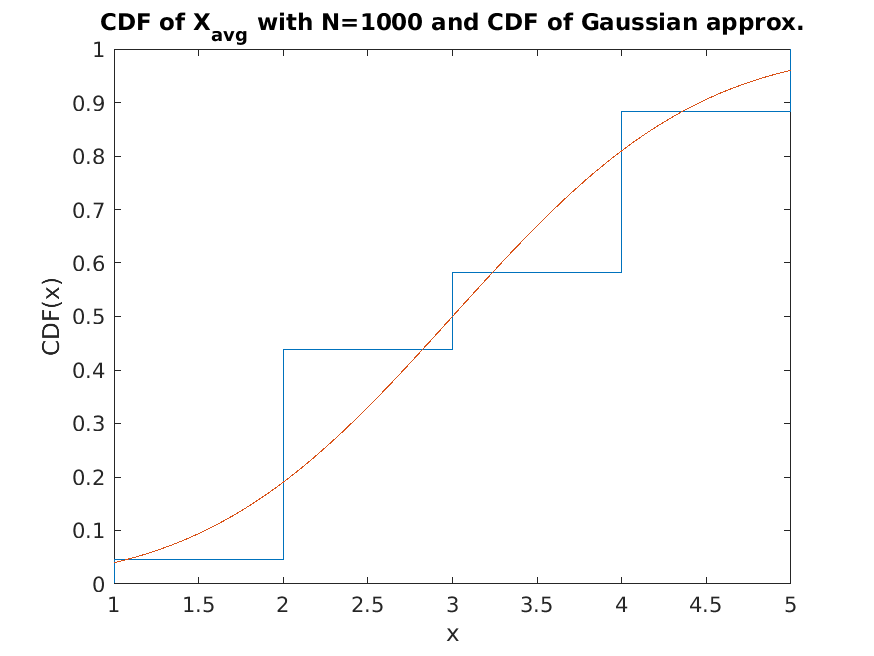
\includegraphics[height=0.4\textwidth]{b_1000.png}}
    \end{floatrow}
    \vspace{1em}
    \begin{floatrow}
        \ffigbox[0.4\textwidth]{}
        {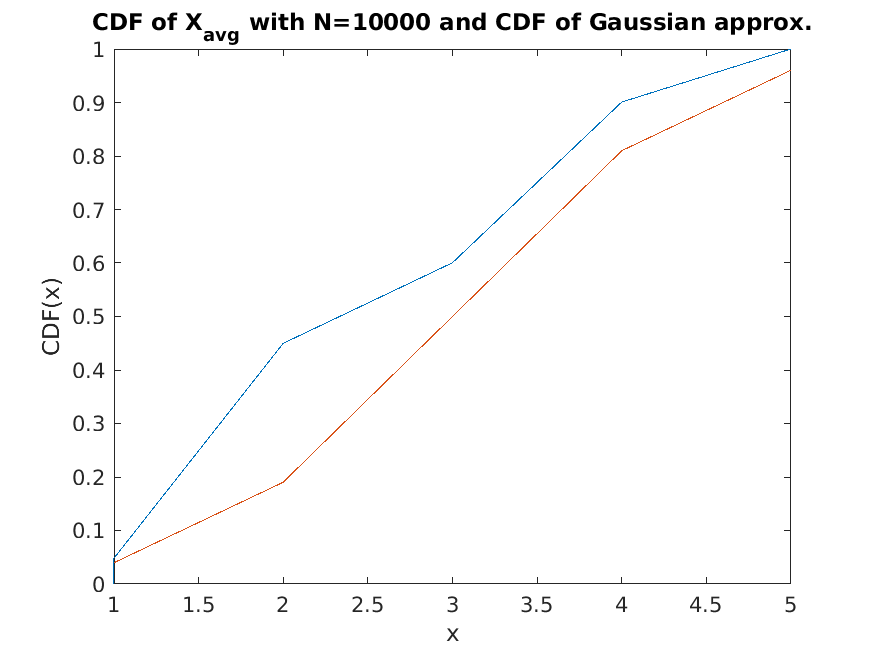
\includegraphics[height=0.4\textwidth]{b_10000.png}}
    \end{floatrow}
\end{figure}

\subsection*{(c)}
\begin{figure}[H]
    \centering
    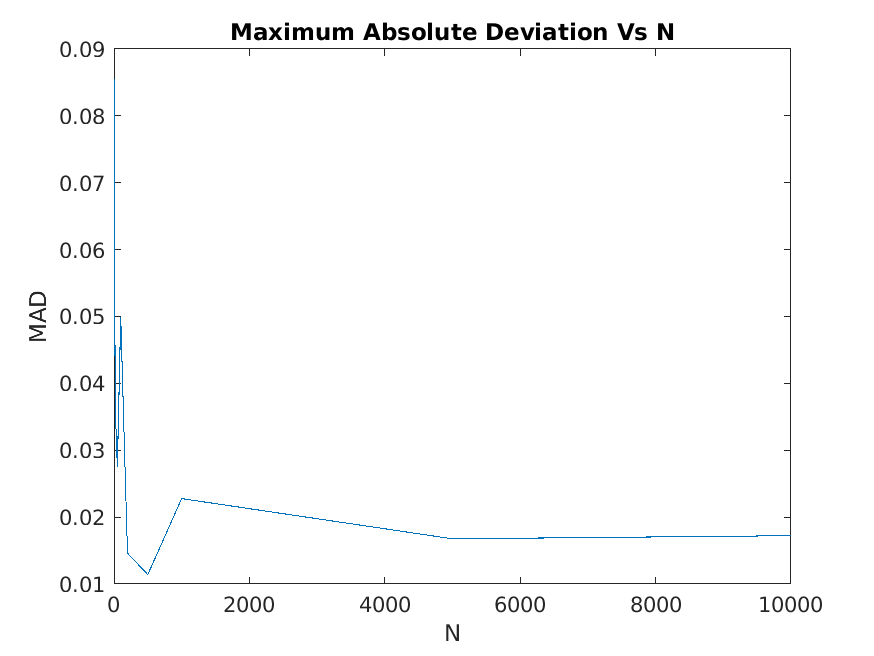
\includegraphics[width=0.8\linewidth]{c.png}
\end{figure}



\newpage
\section*{Question 6}
\addcontentsline{toc}{section}{Question 6}
\setcounter{equation}{0}

\subsection*{Instructions for running the code:}
\begin{itemize}
    \item After extracting submitted file, look for a directory named \texttt{code}. 
    \item Within this, the code for this question is contained in a directory named \texttt{q6} while the 2 images are contained in the \texttt{img} directory.
    \item Run the file \texttt{q6i.m} for plotting the given dependence measures between \texttt{T1.jpg} and \texttt{T2.jpg} and run \texttt{q6ii.m} for plotting the given dependence measures between \texttt{T1.jpg} and it's negative. 
    \item Both of these will create two plots and save them at \texttt{./plots/}
\end{itemize}
\vspace{-1em}
\subsection*{\Large For T1.jpg and T2.jpg}

\begin{figure}[H]
    \centering
    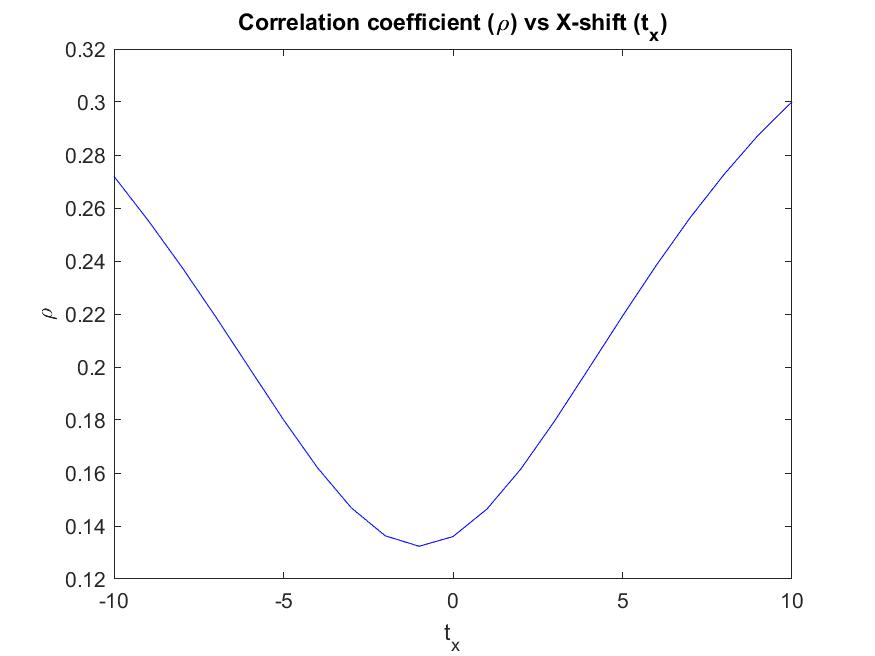
\includegraphics[scale=0.47]{correlation.jpg}
    %\caption{Caption}
    \label{q6ic}
\end{figure}

\subsubsection*{Comments:}
\begin{itemize}
    \item The correlation is the least when the 2 images are almost exactly aligned ($t_x \approx 0$).
    \item As the two images don't seem to have any obvious relation w.r.t their intensity values, thus their correlation coefficient values are low.
    \item As the shift starts to increase in either direction, the images start to become more positively correlated, with the correlation increasing approximately linearly.
    \item The correlation is always positive in the given range of the shifts.
\end{itemize}

\newpage
\begin{figure}[H]
    \centering
    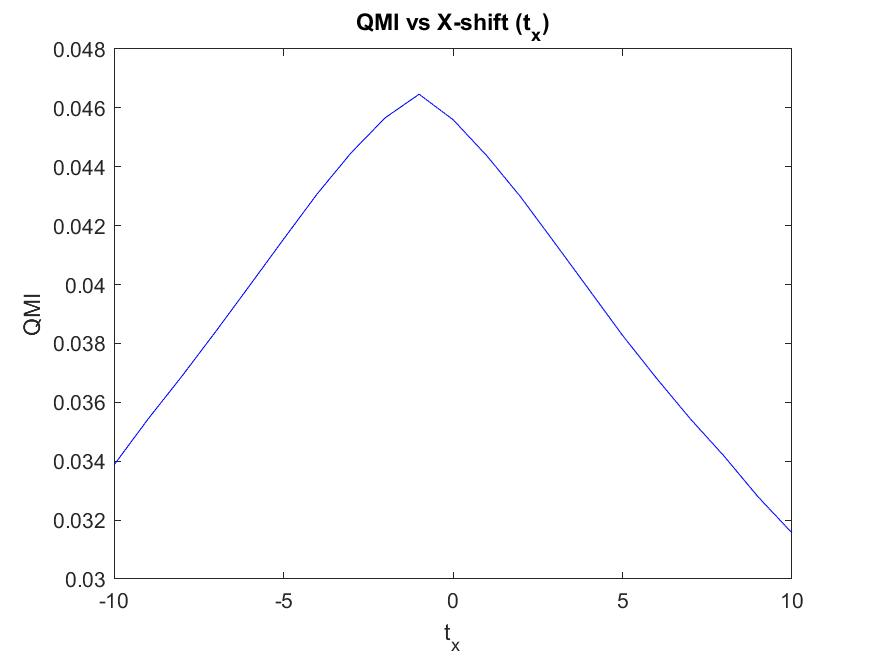
\includegraphics[scale=0.5]{qmi.jpg}
    %\caption{Caption}
    \label{q6ic}
\end{figure}
\subsubsection*{Comments:}
\begin{itemize}
    \item QMI essentially measures the ``dependance" of two random variables on each other. In our case, it is a measure of the mutual information contained between the 2 images.
    \item In our case, the images seem to have no obvious relation  w.r.t their intensity values, thus their QMI values are low.
    \item The QMI value reaches a maximum at $t_x=-1$ (This is also the point where the correlation coefficient is the least)
    \item As we further increase the shift in either direction, the QMI value start decreasing approximately linearly.
\end{itemize}

\newpage
\subsection*{\Large For T1.jpg and it's negative}
\begin{figure}[H]
    \centering
    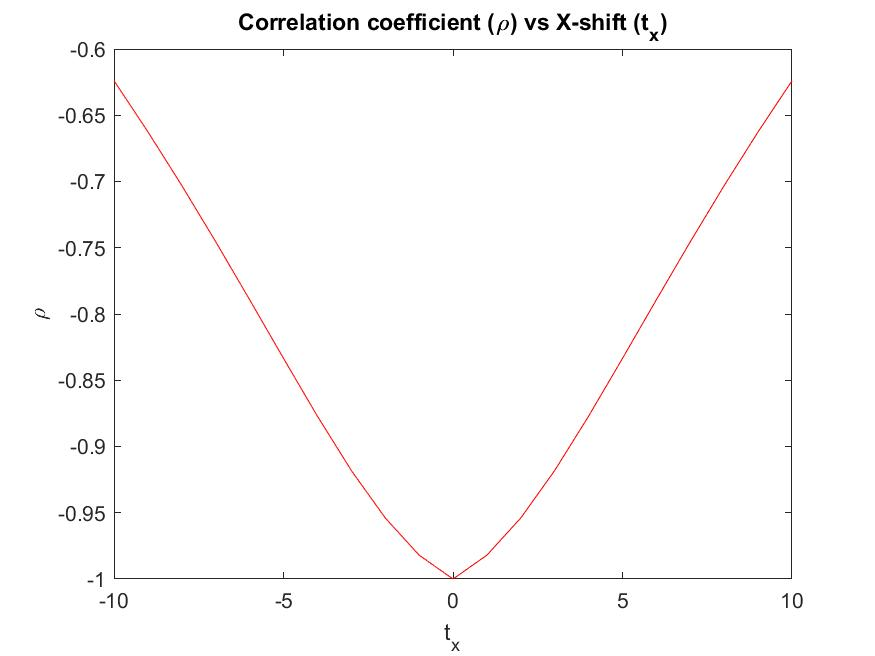
\includegraphics[scale=0.5]{correlation_negative.jpg}
    %\caption{Caption}
    \label{q6ic}
\end{figure}

\subsubsection*{Comments:}
\begin{itemize}
    \item As the second image is the negative of the first and the images are exactly aligned at $t_x = 0$, the correlation coefficient is exactly equal to $(-1)$. Thus, at this point ($t_x = 0$), the two images are completely anti-correlated.
    \item As the shift starts to increase in either direction, the correlation coefficient also starts to become less negative. The increase is approximately linear.
    \item The correlation is always negative in the given range of the shifts for the given image and it's negative.
\end{itemize}


\newpage
\begin{figure}[H]
    \centering
    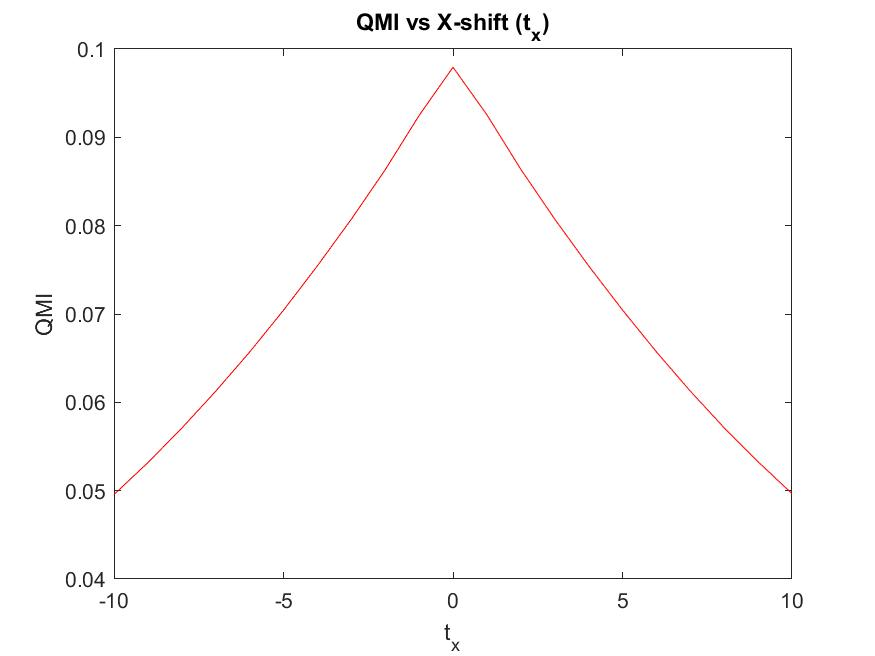
\includegraphics[scale=0.5]{qmi_negative.jpg}
    %\caption{Caption}
    \label{q6ic}
\end{figure}

\subsubsection*{Comments:}
\begin{itemize}
    \item QMI essentially measures the ``dependance" of two random variables on each other. In our case, it is a measure of the mutual information contained between the 2 images.
    \item In our case, the second image is the negative of the first, thus both of them contain the exact same information about each other at $t_x = 0.$ ($(255 - I_1 = I_2) \text{ and } (255-I_2) = I_1$)
    \item As we increase the shift in either direction, the QMI values start to decrease, as when we are shifting an image, we are also ``deleting" information by blacking out the un-occupied pixels.
    \item The rate of decrease of QMI is higher in this case as compared to the previous case.
    \item Although the QMI values appear quite low at $t_x = \pm 10$, these are still higher than the previous case, where the maxima itself was about $0.046$. This is because even after deleting some information from the negative, there is still a lot of common information between the 2 images.
\end{itemize}




\newpage
\section*{Question 7}
\addcontentsline{toc}{section}{Question 7}
\setcounter{equation}{0}

MGF of Multinomial distribution of $\mathbf{X} = (X_1, \dots, X_k)$, where $\sum_{i=1}^{k} X_i = n$ is $\phi_{\mathbf{X}}(\mathbf{t}) = (p_1 e^{t_1} + \cdots + p_k e^{t_k})^{n}$, where $\mathbf{t} = (t_1, \dots, t_k)$ and $p_i$ represent probability of $X_i$. \\
\begin{equation*}
    \begin{split}
        \frac{\partial}{\partial t_i} \phi_{\mathbf{X}}(\mathbf{t}) &= n \cdot (p_1 e^{t_1} + \cdots + p_k e^{t_k})^{n-1} \cdot (p_i e^{t_i}) \\
        \mu_i = E(X_i) &= \frac{\partial}{\partial t_i} \phi_{\mathbf{X}}(\mathbf{t}) \bigg\rvert_{\mathbf{t} = \mathbf{0} = (0, \dots, 0)} \\
            &= n \cdot (p_1 + \cdots + p_k)^{n-1} \cdot p_i \\
            &= n \cdot p_i \hspace{3em} (\sum_{n=1}^{k} p_i = 1) 
    \end{split}
\end{equation*}

\begin{equation*}
    \begin{split}
        \frac{\partial^2}{\partial t_i^2} \phi_{\mathbf{X}}(\mathbf{t}) &= n(n-1) \cdot (p_1 e^{t_1} + \cdots + p_k e^{t_k})^{n-2} \cdot (p_i e^{t_i})^2 + n \cdot (p_1 e^{t_1} + \cdots + p_k e^{t_k})^{n-1} \cdot (p_i e^{t_i}) \\
        E(X_i^2) &= \frac{\partial^2}{\partial t_i^2} \phi_{\mathbf{X}}(\mathbf{t}) \bigg\rvert_{\mathbf{t} = \mathbf{0} = (0, \dots, 0)} \\
            &= n(n-1) \cdot (p_1 + \cdots + p_k)^{n-2} \cdot p_i^2 + n \cdot (p_1 + \cdots + p_k)^{n-1} \cdot p_i \\
            &= n(n-1) \cdot p_i^2 + n \cdot p_i \hspace{3em} (\sum_{n=1}^{k} p_i = 1) \\
        Cov(X_i, X_i) &= Var(X_i) \\
            &= E(X_i^2) - E(X_i)^2 \\
            &= n(n-1) \cdot p_i^2 + n \cdot p_i - (n \cdot p_i)^2 \\
            &= n \cdot p_i (1 - p_i) \\
    \end{split}
\end{equation*}

For $i \ne j$,
\begin{equation*}
    \begin{split}
        \frac{\partial^2}{\partial t_j \partial t_i} \phi_{\mathbf{X}}(\mathbf{t}) &= n(n-1) \cdot (p_1 e^{t_1} + \cdots + p_k e^{t_k})^{n-2} \cdot (p_i e^{t_i}) \cdot (p_j e^{t_j}) \\
        E(X_i \cdot X_j) &= \frac{\partial^2}{\partial t_j \partial t_i} \phi_{\mathbf{X}}(\mathbf{t}) \bigg\rvert_{\mathbf{t} = \mathbf{0} = (0, \dots, 0)} \\
            &= n(n-1) \cdot (p_1 + \cdots + p_k)^{n-2} \cdot p_i \cdot p_j \\
            &= n(n-1) \cdot p_i  \cdot p_j \hspace{3em} (\sum_{n=1}^{k} p_i = 1) \\
        Cov(X_i, X_j) &= E[(X_i - \mu_i)(X_j - \mu_j)] \\
            &= E[(X_i - E(X_i))(X_j - E(X_j))] \\
            &= E(X_i \cdot X_j) - E(X_i)E(X_j) \\
            &= n(n-1) \cdot p_i  \cdot p_j - (n \cdot p_i)(n \cdot p_j) \\
            &= (-n) \cdot p_i \cdot p_j  \\
    \end{split}
\end{equation*}

The co-variance matrix $\mathbf{C}$ of $\mathbf{X}$ is given by:
\begin{equation*}
    \begin{split}
        C_{ii} &= n \cdot p_i (1 - p_i) \\
        C_{ij} &= (-n) \cdot p_i \cdot p_j \quad \forall \ i \ne j \\
    \end{split}
\end{equation*}


\end{document}

